\documentclass[12pt]{article}\usepackage[margin=1in]{geometry}\usepackage{amsmath,amssymb,amsthm,graphicx,natbib,microtype}\newtheorem{theorem}{Theorem}\newtheorem{corollary}[theorem]{Corollary}
\title{Combined Directional Support Transfer\\\large Rayleigh Forcing, Frame Volume, Leading Scale, and Capacity in One Bound}\author{Prime Dynamics Theory Program}\date{July 2026}
\begin{document}\maketitle
\begin{abstract}
We combine RH-120, RH-123, and RH-124 into one directional support theorem.
Let $V=\sqrt{\det G}$ and
$B=(1-\gamma)_+^4V/(L^4C)$.  If the gauged next level has retained Gram
$a(1-\eta)$, tail parameters $b,\delta$, determinant $|\det S|$, leading
factor $\ell$, and capacity factor $c$, then with
\[
\widehat\gamma'^2=\frac{b\gamma^2+\delta}{a(1-\eta)}
\]
we have
\[
B'\geq\frac{[a(1-\eta)]^2|\det S|}{\ell^4c}
(1-\widehat\gamma')_+^4\frac{V}{L^4C}.
\]
The formula is sharp when every input inequality is an equality.  On the
explicitly conditioned RH-121 archive, all 96 one-step transfers are
nonzero and all 24 five-scale chains finish above $10^{-8}$.  The audit is a
regularized consistency test, not a physical or asymptotic support proof.
\end{abstract}
\section{The combined candidate}
The RH-114 directional lower, after RH-110 capacity division, is
\[
B(G,D;L,C)=\frac{(1-\gamma(G,D))_+^4\sqrt{\det G}}{L^4C}.
\]
All factors must refer to the same enclosed operator.  Treating them as
independent black boxes can lose the correlation quantified in RH-124.

\begin{theorem}[Combined directional transfer]\label{thm:combined}
Assume the RH-123 hypotheses
\[
G'\succeq a(1-\eta)S^*GS,qquad
D'\preceq bS^*DS+\delta S^*GS,
\]
and suppose $L'\leq\ell L$ and $C'\leq cC$.  Define
$\widehat\gamma'^2=(b\gamma^2+\delta)/[a(1-\eta)]$.  In four dimensions,
\[
B'\geq \frac{[a(1-\eta)]^2|\det S|}{\ell^4c}
(1-\widehat\gamma')_+^4\frac{\sqrt{\det G}}{L^4C}.
\]
\end{theorem}
\begin{proof}
RH-123 gives $\gamma'\leq\widehat\gamma'$.  Determinant monotonicity gives
$\sqrt{\det G'}\geq[a(1-\eta)]^2|\det S|\sqrt{\det G}$.  Insert these three
one-sided inequalities into the definition of $B'$.
\end{proof}
These are standard positive-matrix and singular-value operations
\citep{Bhatia2007,HornJohnson1991}.  Equality is attained by scalar relative
tails, exact Gram scaling, and exact choices $L'=\ell L$, $C'=cC$.

\begin{corollary}[Iterated lower]
If the one-step theorem gives $B_{n+1}\geq m_nB_n$, then
$B_N\geq B_0\prod_{n<N}m_n$.  Any independently established lower for
$B_0$ may replace the exact source value.
\end{corollary}

\section{Five-scale conditioned audit}
We apply the exact-Gram gauges from RH-121 to 96 adjacent-scale pairs.  Thus
$a=1$, $\eta=\delta=0$, $b=b_{\rm opt}$, while $\ell$ and $c$ are the
observed ratios of the archived leading and capacity uppers.  Every target
lower is compared with the target candidate computed on the same
regularized Gram path.

There are zero one-step dominance failures.  All 96 transfers are nonzero;
95 exceed $10^{-8}$.  Grouping by side, threshold, and normalized phase gives
24 chains.  Their terminal lowers range from $1.13\times10^{-7}$ to
$8.27\times10^{-2}$, with median $2.59\times10^{-2}$.  All 24 exceed
$10^{-8}$, 23 exceed $10^{-6}$, and 21 exceed $10^{-4}$.
\begin{figure}[h]\centering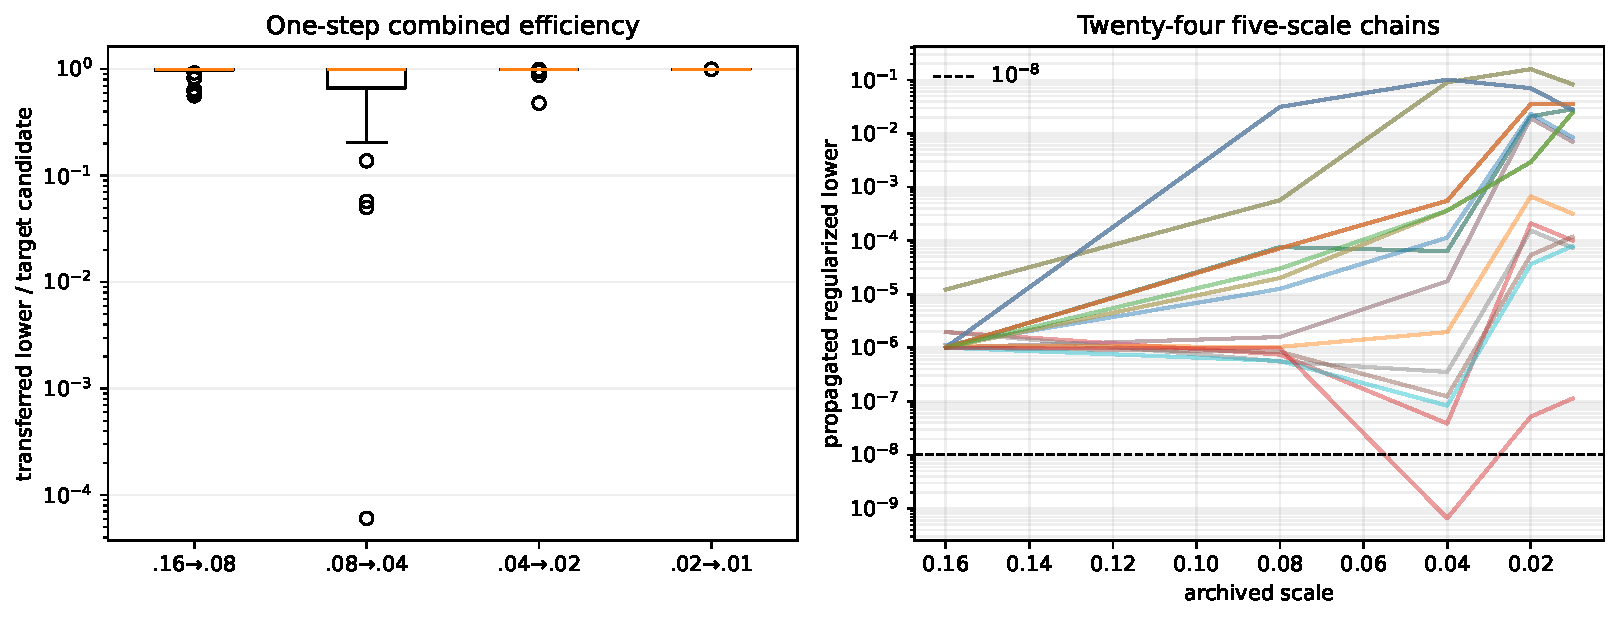
\includegraphics[width=\textwidth]{figures/combined_directional_support_transfer.pdf}\caption{One-step efficiency and iterated regularized lower chains.}\end{figure}

The good finite propagation does not erase the RH-121 boundary.  Its
$10^{-12}$ Gram conditioning floor is not a physical lower enclosure, so
these chains cannot be promoted to support certificates.  RH-126 develops
the independent direct-margin fallback; RH-127 supplies outward guards.
No uniform Stage A, Hilbert--Polya operator, zeta-zero identification, or
Riemann Hypothesis conclusion is claimed.
\bibliographystyle{plainnat}\bibliography{references}\end{document}
